% Diagram of Android activity life cycle
% Author: Pavel Seda 
\documentclass[border=10pt]{standalone}
\usepackage{tikz}
\usetikzlibrary{arrows.meta}
\usetikzlibrary{calc}
\tikzset{%
  >={Latex[width=2mm,length=2mm]},
  % Specifications for style of nodes:
            base/.style = {rectangle, rounded corners, draw=black,
                           minimum width=4cm, minimum height=1cm,
                           text centered, font=\sffamily},
  activityStarts/.style = {base, fill=blue!30},
       startstop/.style = {base, fill=red!30},
    activityRuns/.style = {base, fill=green!30},
         process/.style = {base, minimum width=2.5cm, fill=orange!15,
                           font=\ttfamily},
}
\begin{document}    
% Drawing part, node distance is 1.5 cm and every node
% is prefilled with white background
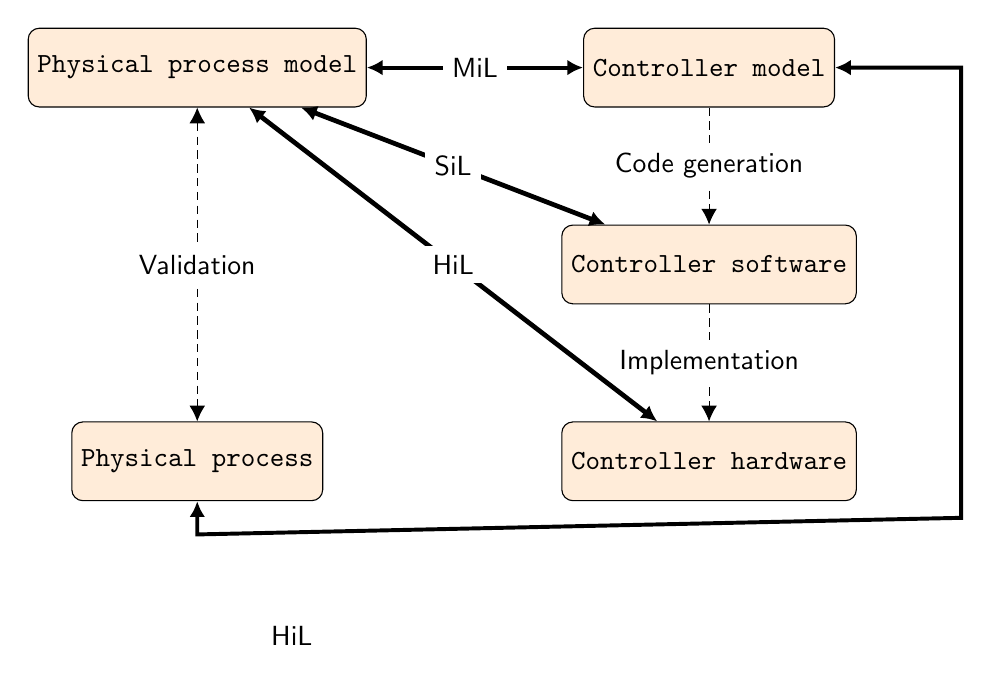
\begin{tikzpicture}[node distance=1.5cm,
    every node/.style={fill=white, font=\sffamily}, align=center]
  % Specification of nodes (position, etc.)
  
  
  \node (controllerMdl) [process] {Controller model};
  \node (controllerSw)  [process, below of=controllerMdl, yshift=-1cm] {Controller software};
  \node (controllerHw)    [process, below of=controllerSw, yshift=-1cm] {Controller hardware};
  \node (proceMdl)    [process, left of=controllerMdl, xshift=-5cm] {Physical process model};
	\node (proce)    [process, left of=controllerHw, xshift=-5cm] {Physical process};
     
  % Specification of lines between nodes specified above
  % with aditional nodes for description 

  \draw[->,densely dashed] (controllerMdl) -- node {Code generation} (controllerSw);
	\draw[->,densely dashed] (controllerSw) -- node {Implementation} (controllerHw);
	\draw[<->,densely dashed] (proceMdl) -- node {Validation} (proce);
	
	\draw[<->,line width=0.5mm] (controllerMdl) -- node {MiL} (proceMdl);
	\draw[<->,line width=0.6mm] (controllerSw) -- node {SiL} (proceMdl);
	\draw[<->,line width=0.6mm] (controllerHw) -- node {HiL} (proceMdl);
	
	\coordinate (A) at ($(controllerMdl.east) + (1.6,0)$);
	\path let \p1=(A), \p2=(proce.south) in coordinate (B) at (\x1,-6+\y2);
	\path let \p3=(B), \p2=(proce.south) in coordinate (C) at (\x2,-6+\y3);
	
	
	
	\draw[<->,line width=0.5mm] (controllerMdl.east) -- (A)  -- (B) -- (C) -- 
								node[ xshift=1.2cm,yshift=-1.5cm,text width=2.5cm]
     {HiL}(proce.south)
      ;
  
  \end{tikzpicture}
\end{document}